\documentclass{article}
\usepackage{graphicx}
\title{PileUp Rejection Criteria based on BBC}
\author{Carlos Perez Lara\and Jaehyeon Do \and Veronica Canoa Roman}
\date{Last updated: \today}

\begin{document}
\maketitle

\section{The BBC detector}
The BBC detector provides information about the centrality and time of the collision.
Each arm (south and north) read from 64 photomultiplier tubes with both charge and time ifnormation.
The procedure for calibration of the signal is equal since RunXX and it is documented somewhere else \cite{A}.
Here we investigate the usage of the TDC signals to formulate a event selection that prevents the analysis of pileup events.

\section{The BBC timing coincidence}
\begin{figure}
\centering
\includegraphics[width=0.48\textwidth]{fig_pileup/dAu200MB_rmsSouth_455547}\hfil
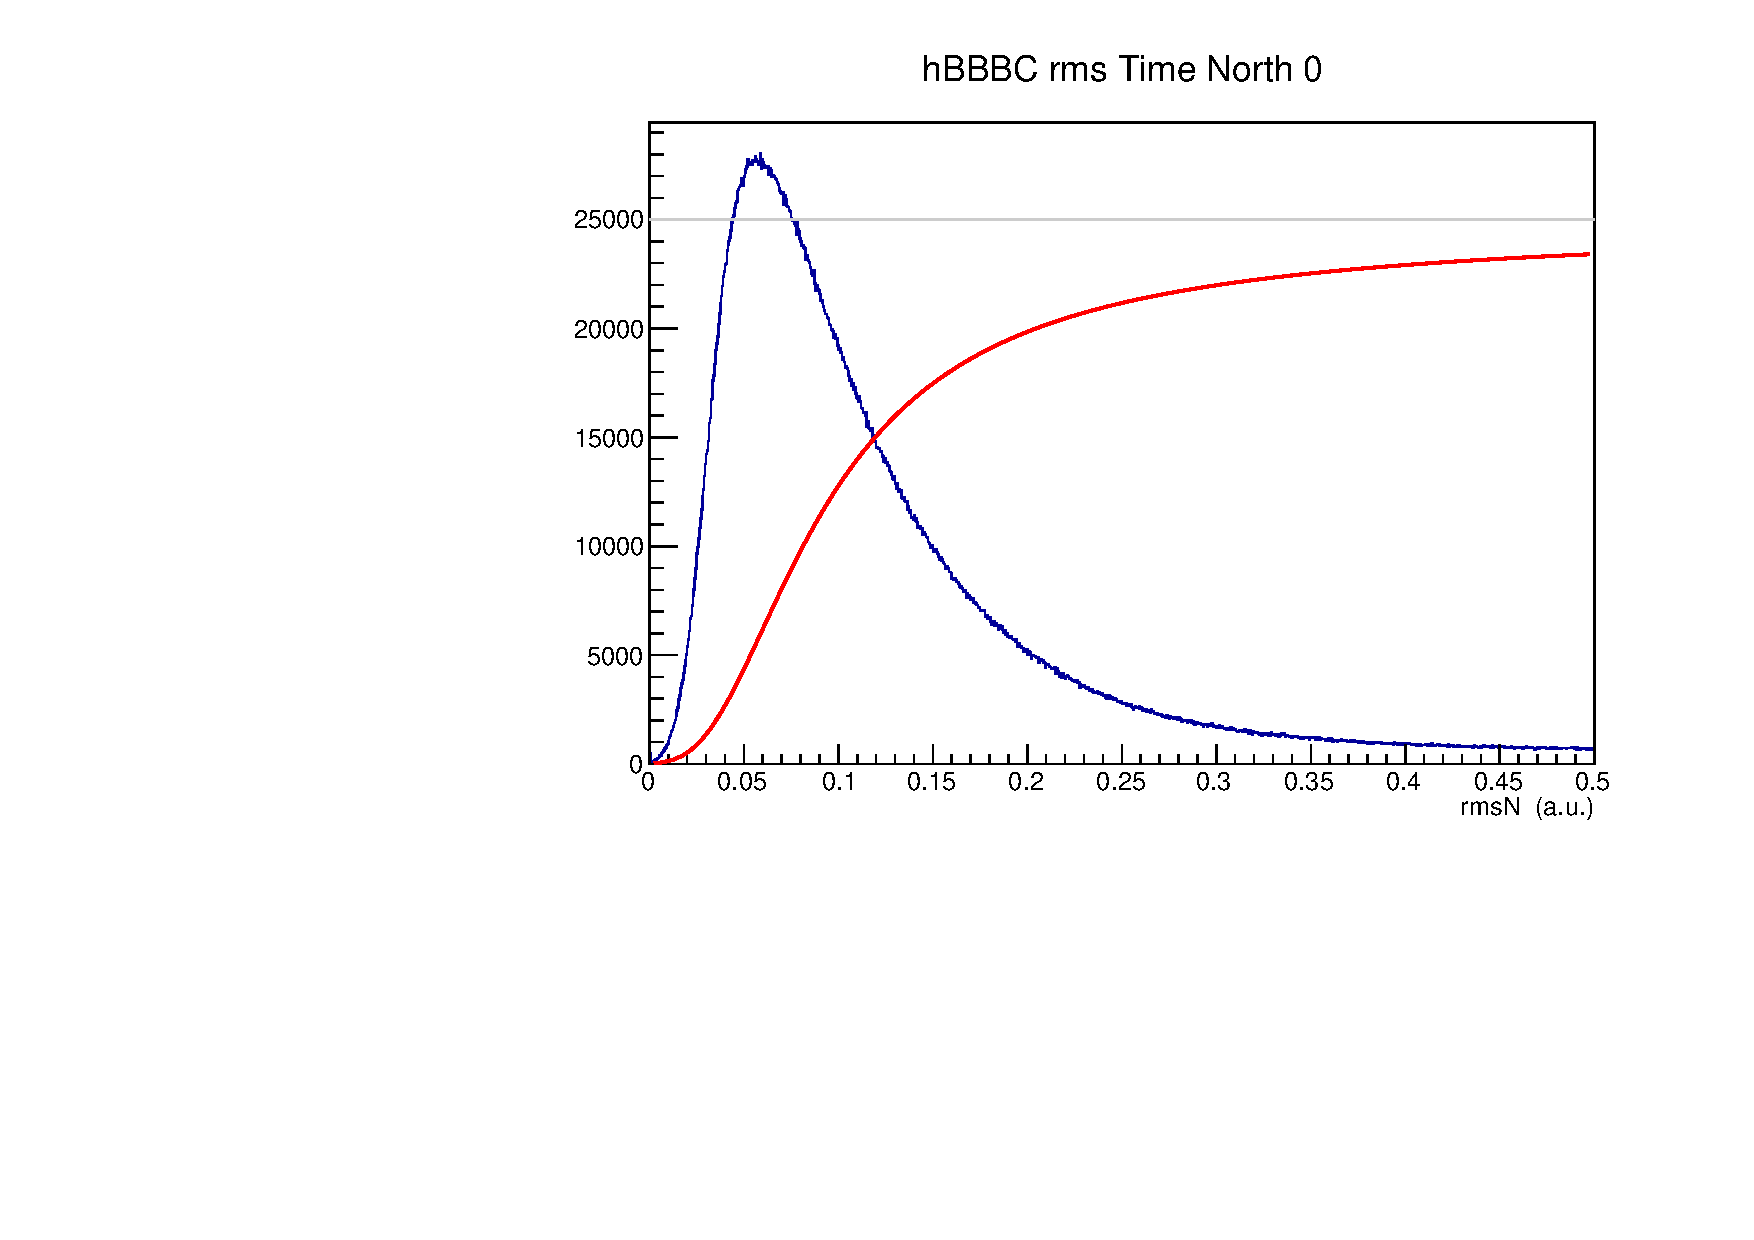
\includegraphics[width=0.48\textwidth]{fig_pileup/dAu200MB_rmsNorth_455547}\\
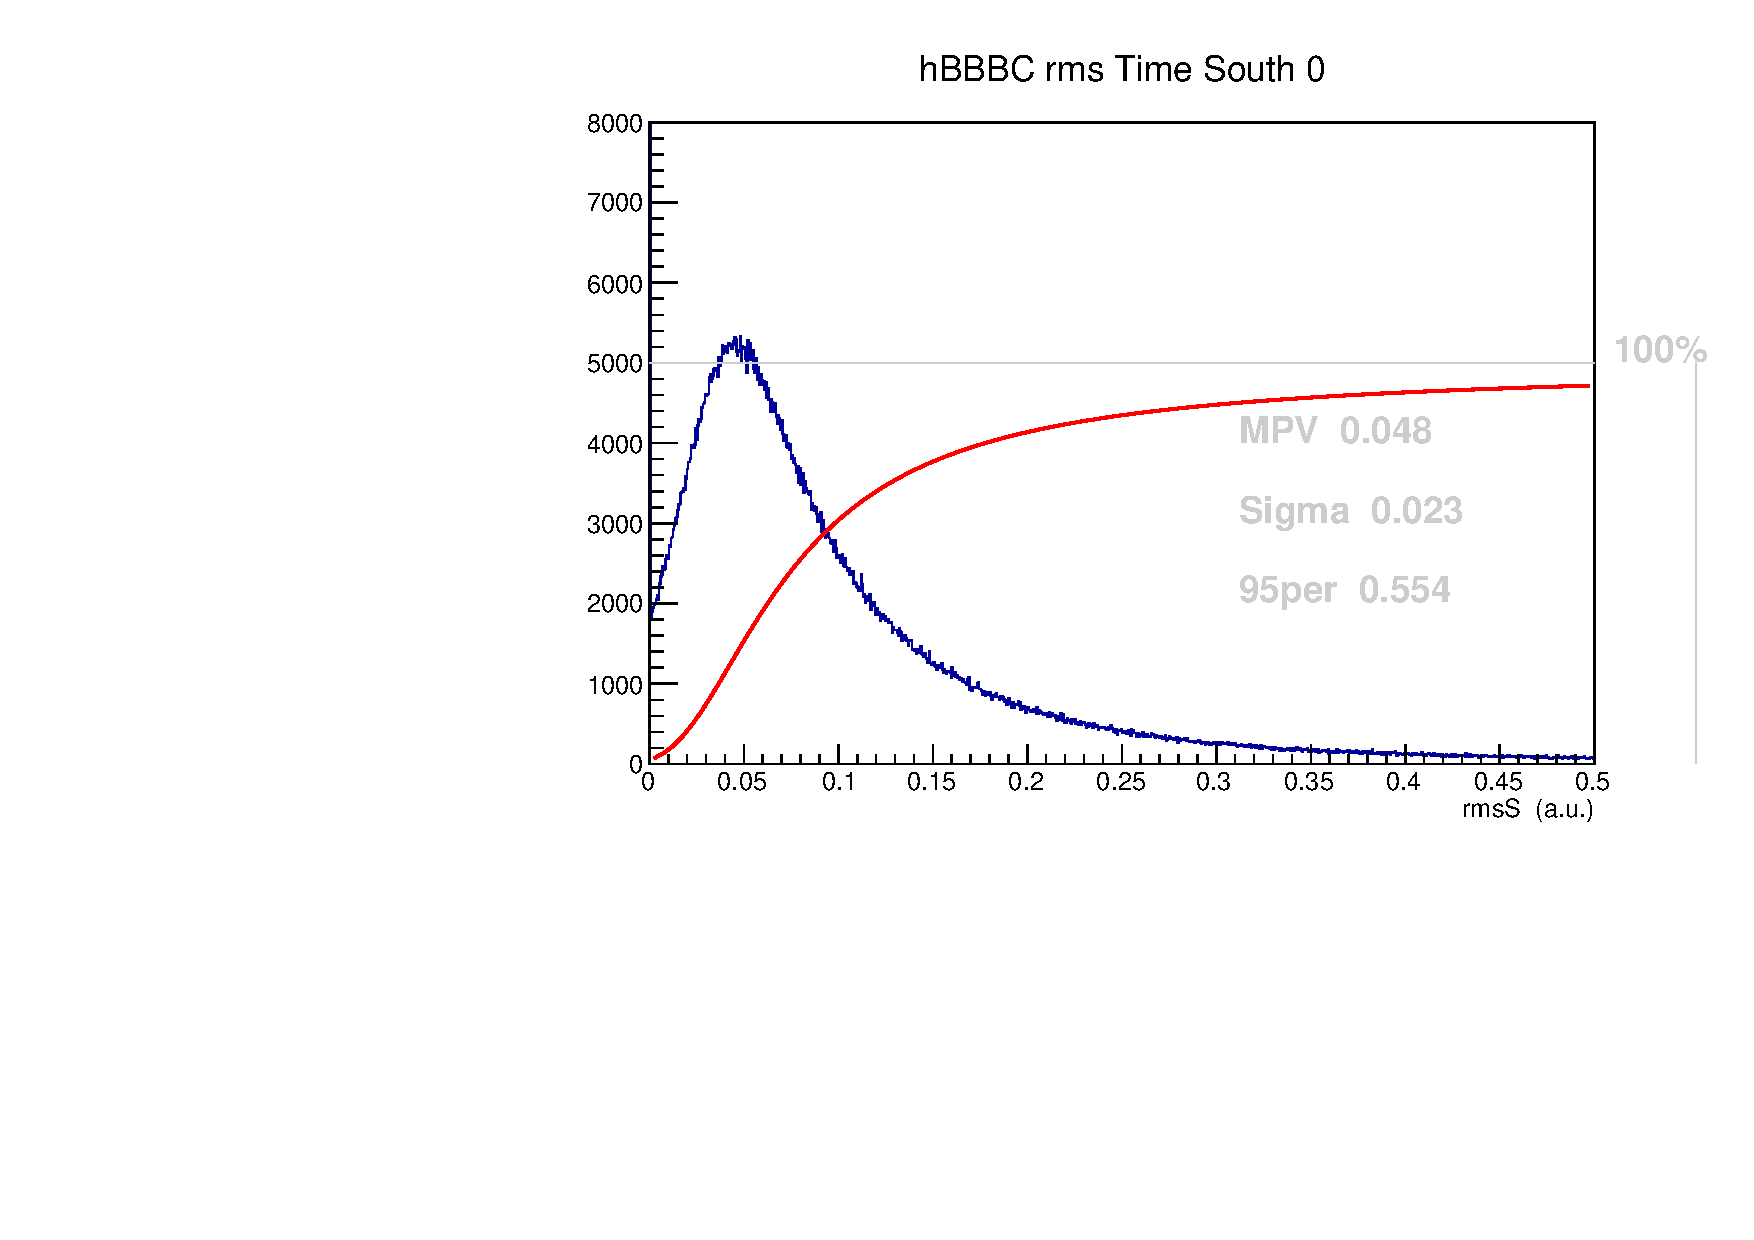
\includegraphics[width=0.48\textwidth]{fig_pileup/pp200_rmsSouth_431739}\hfil
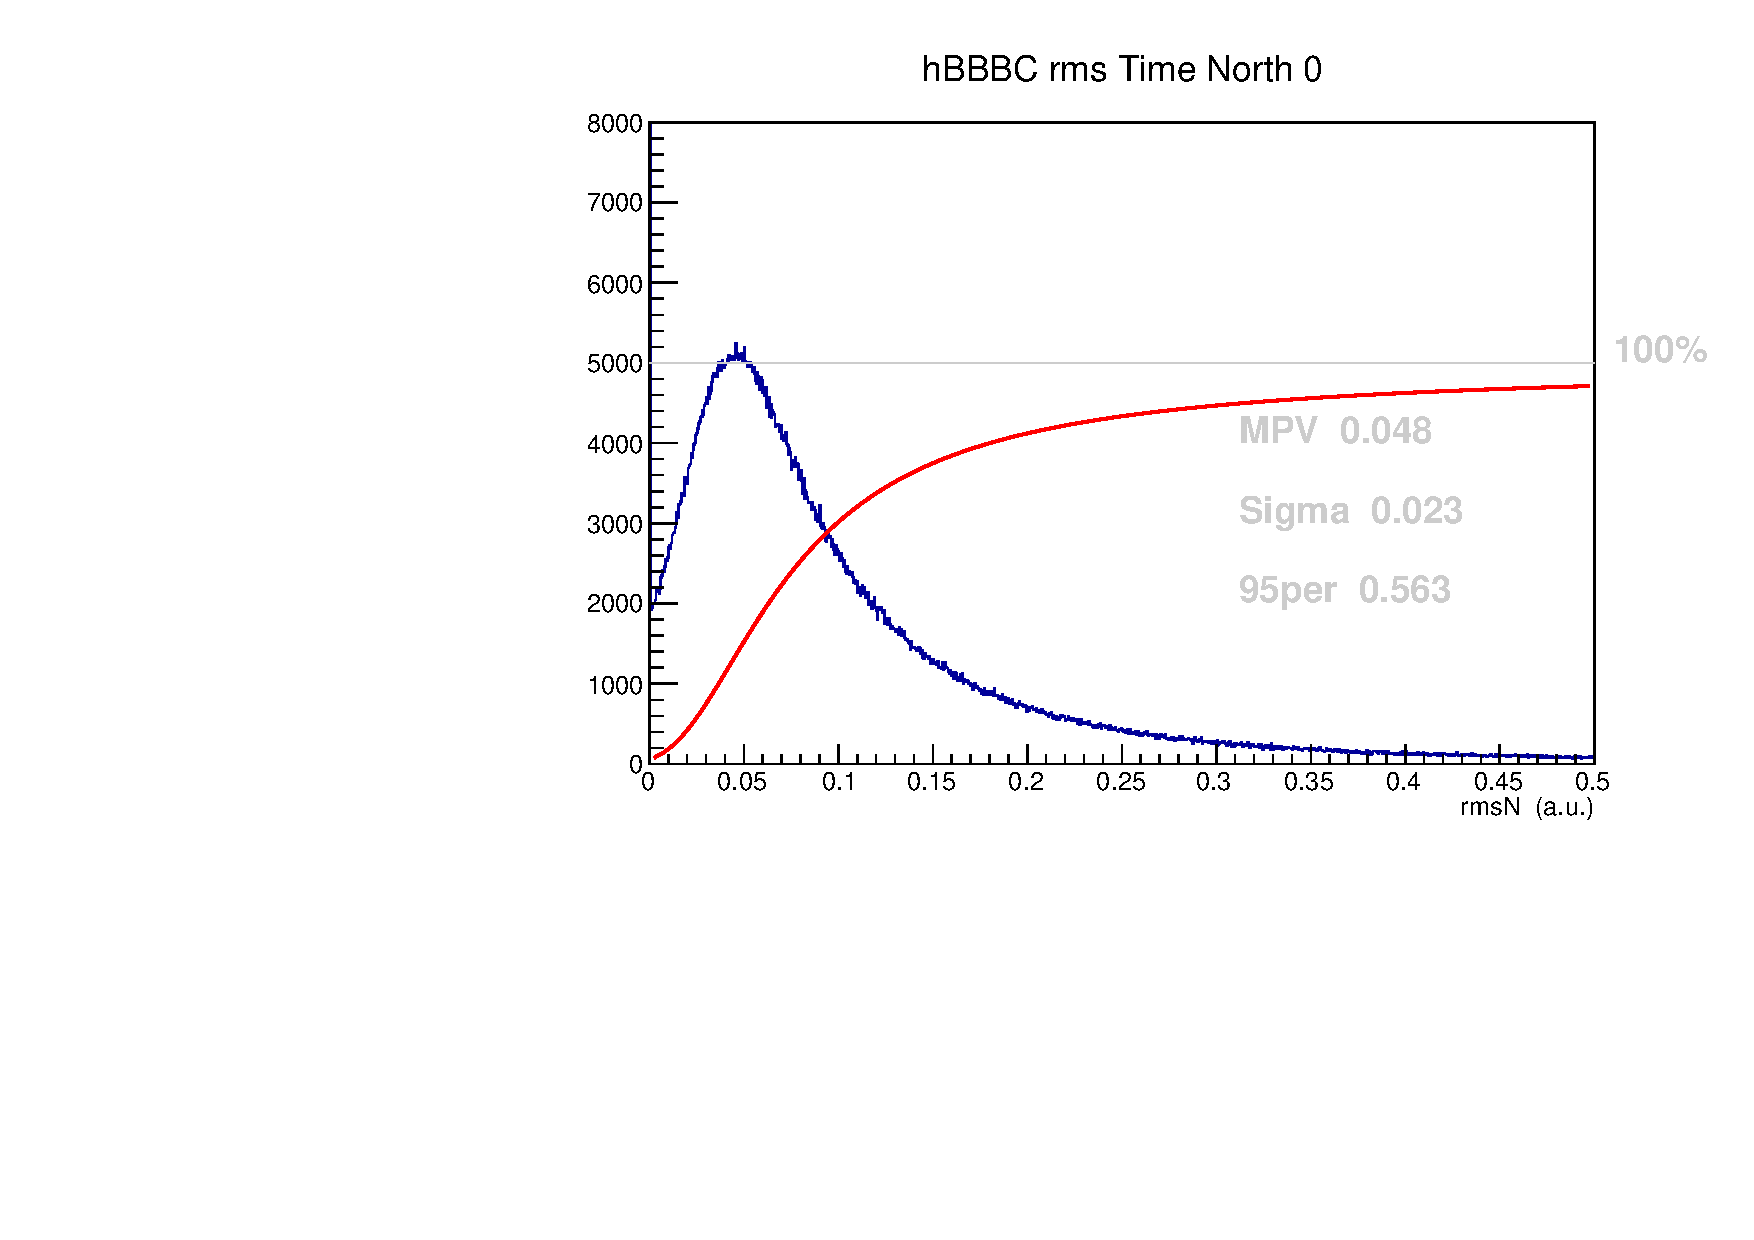
\includegraphics[width=0.48\textwidth]{fig_pileup/pp200_rmsNorth_431739}
\label{fig.dau200mb.bbctimetime}
\caption{Raw distribution of time coincidence for BBC in dAu collisions from 0 to 5 \% centrality at 200 GeV. Each pannel represents situation for one run.}
\end{figure}
For each arm we take the RMS of the 64 time signal weighted by their charge.
Figure \ref{fig.dau200mb.bbctimetime} shows the rms distribution for both south (left) and north (right) arm. The top panels correspond to one of the d+Au dataset where a centrality selection of 0-5\% was applied.
As one can see the distributions are quite similar for the d-going and Au-going direction.
The distribution can be approximated to a Landau distribution and estimate its peak position and width.
The parameters of the fit are reported in the figures.
Notice that for dAu the mean of the fit does not vary much from south to north, however the sigma is quite different.


\section{Run16 dAu 200 GeV}
\begin{figure}
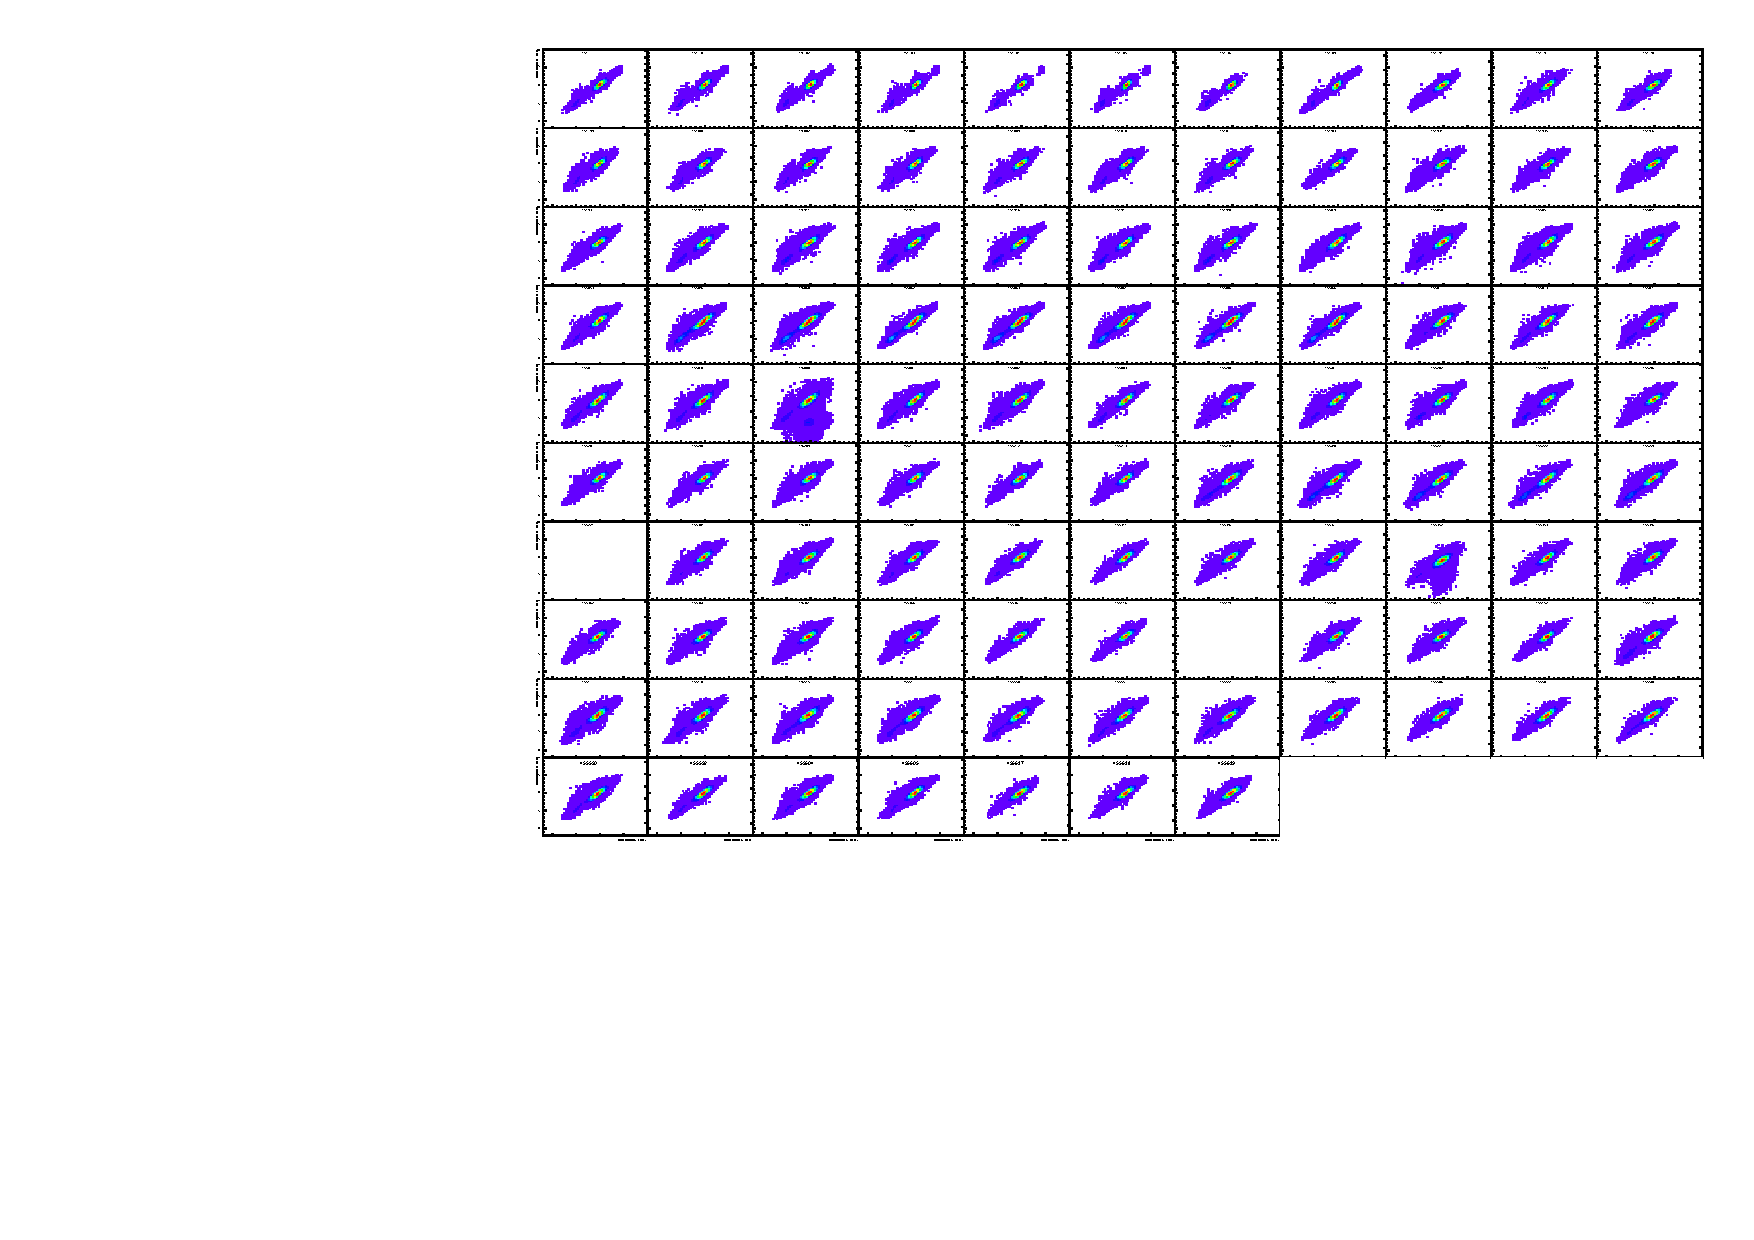
\includegraphics[width=\textwidth]{fig_pileup/dAu200MB_TimingBBC_TimeTimeBC}\\
\label{fig.dau200mb.bbctimetime}
\caption{Raw distribution of time coincidence for BBC in dAu collisions from 0 to 5 \% centrality at 200 GeV. Each pannel represents situation for one run.}
\end{figure}

\begin{figure}
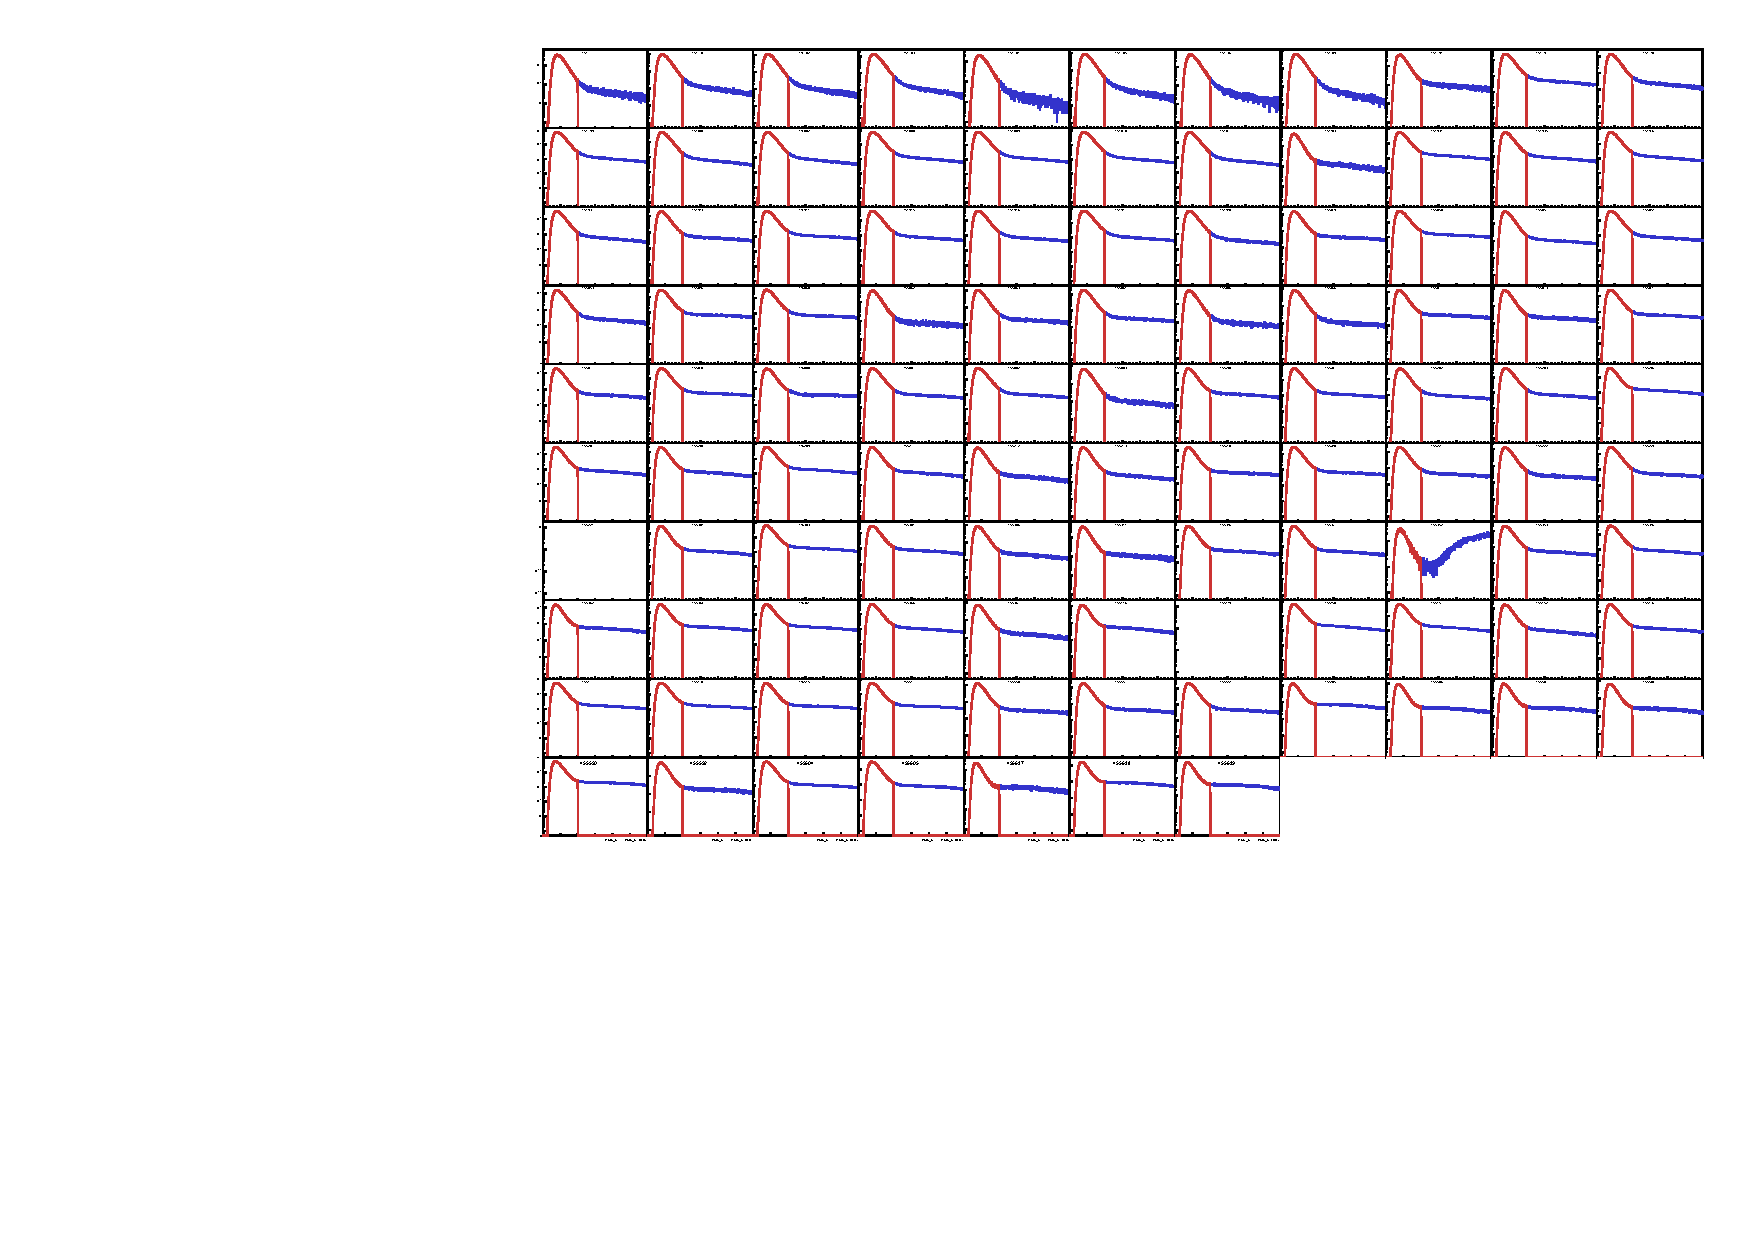
\includegraphics[width=\textwidth]{fig_pileup/dAu200MB_TimingBBC_RMS}
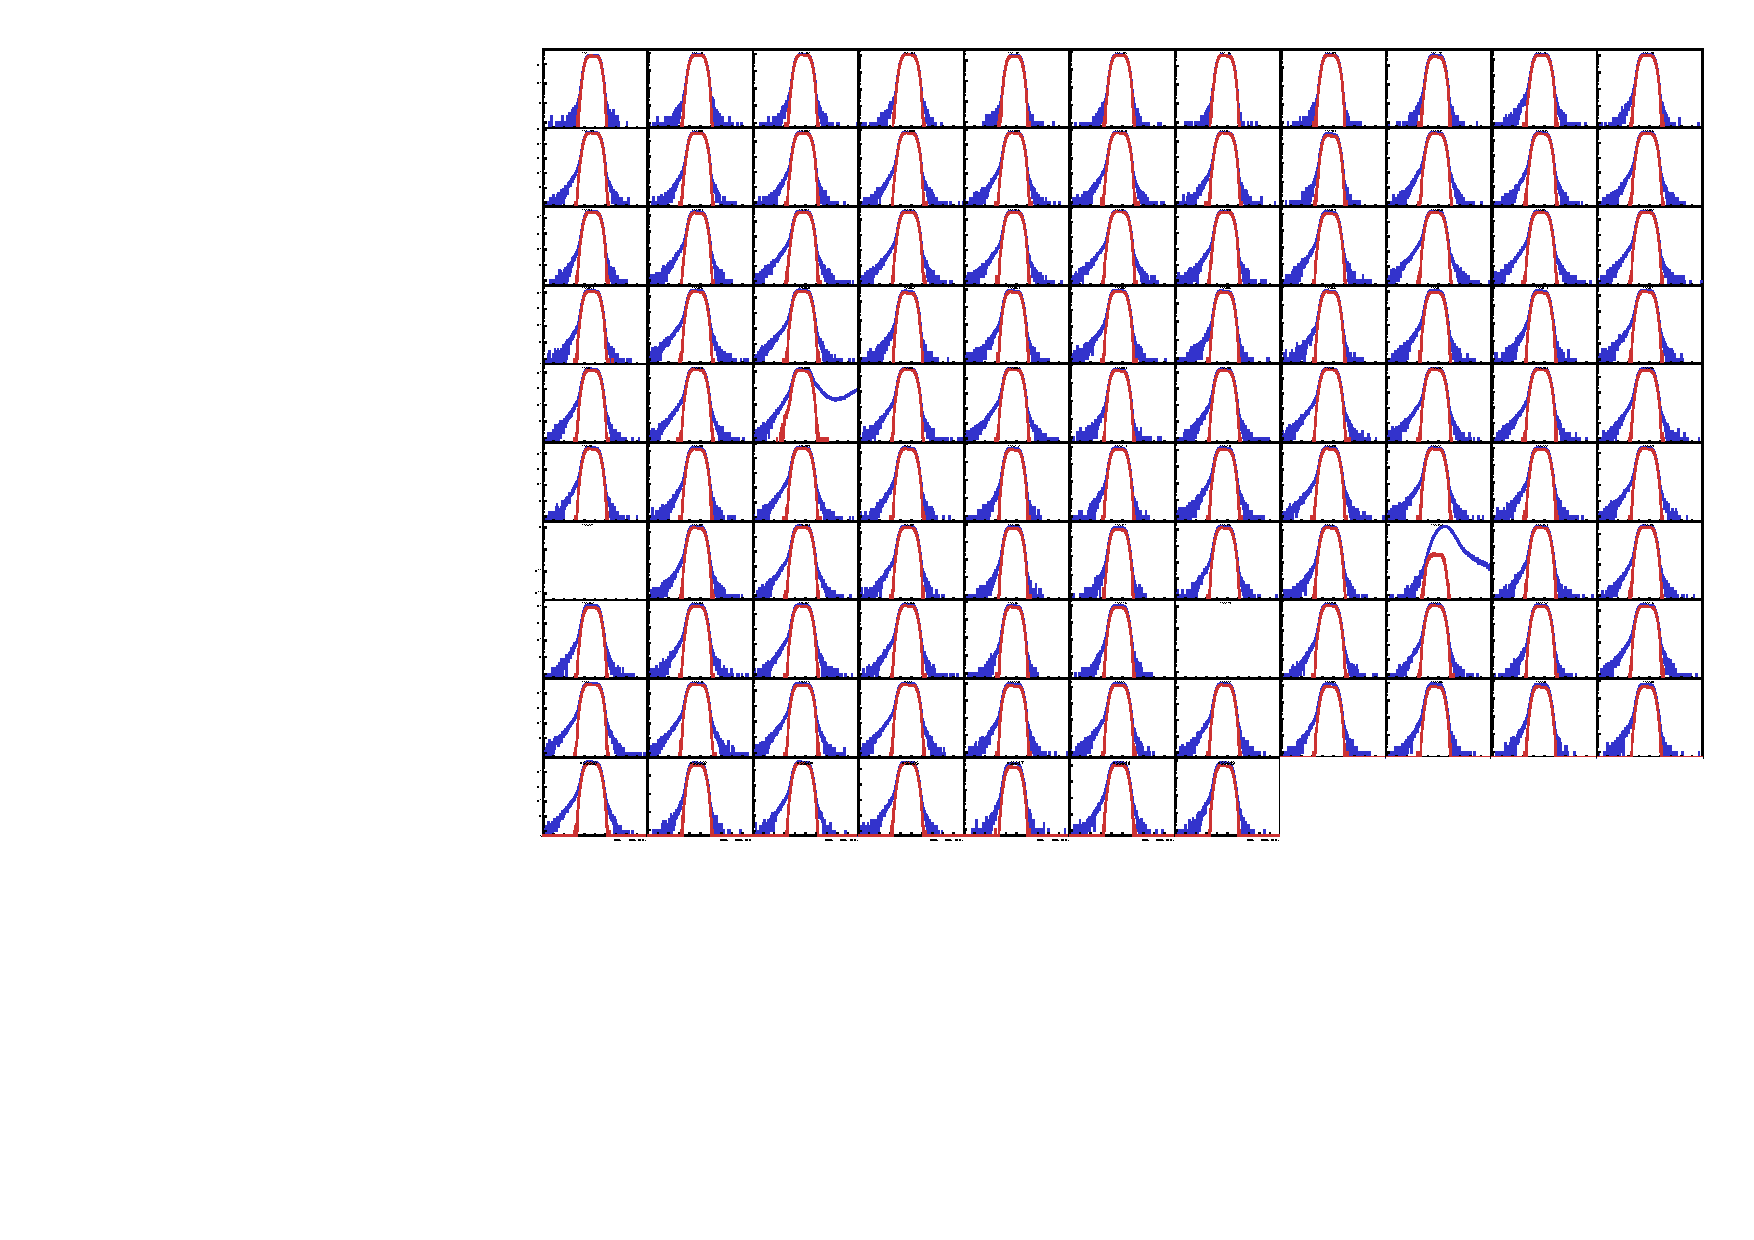
\includegraphics[width=\textwidth]{fig_pileup/dAu200MB_TimingBBC_Time}
\label{fig.dau200mb.bbctimetime}
\caption{Performance of BBC timing cut  in dAu collisions from 0 to 5 \% centrality at 200 GeV. Each pannel represents situation for one run. The bottom plot corresponds to the difference between the north and south estimation of time event-by-event , while the top plot corresponds to the RMS within the south arm. The blue distributions are for the variables before the coincidence cut. The red distributions are after the cut.}
\end{figure}

\begin{figure}
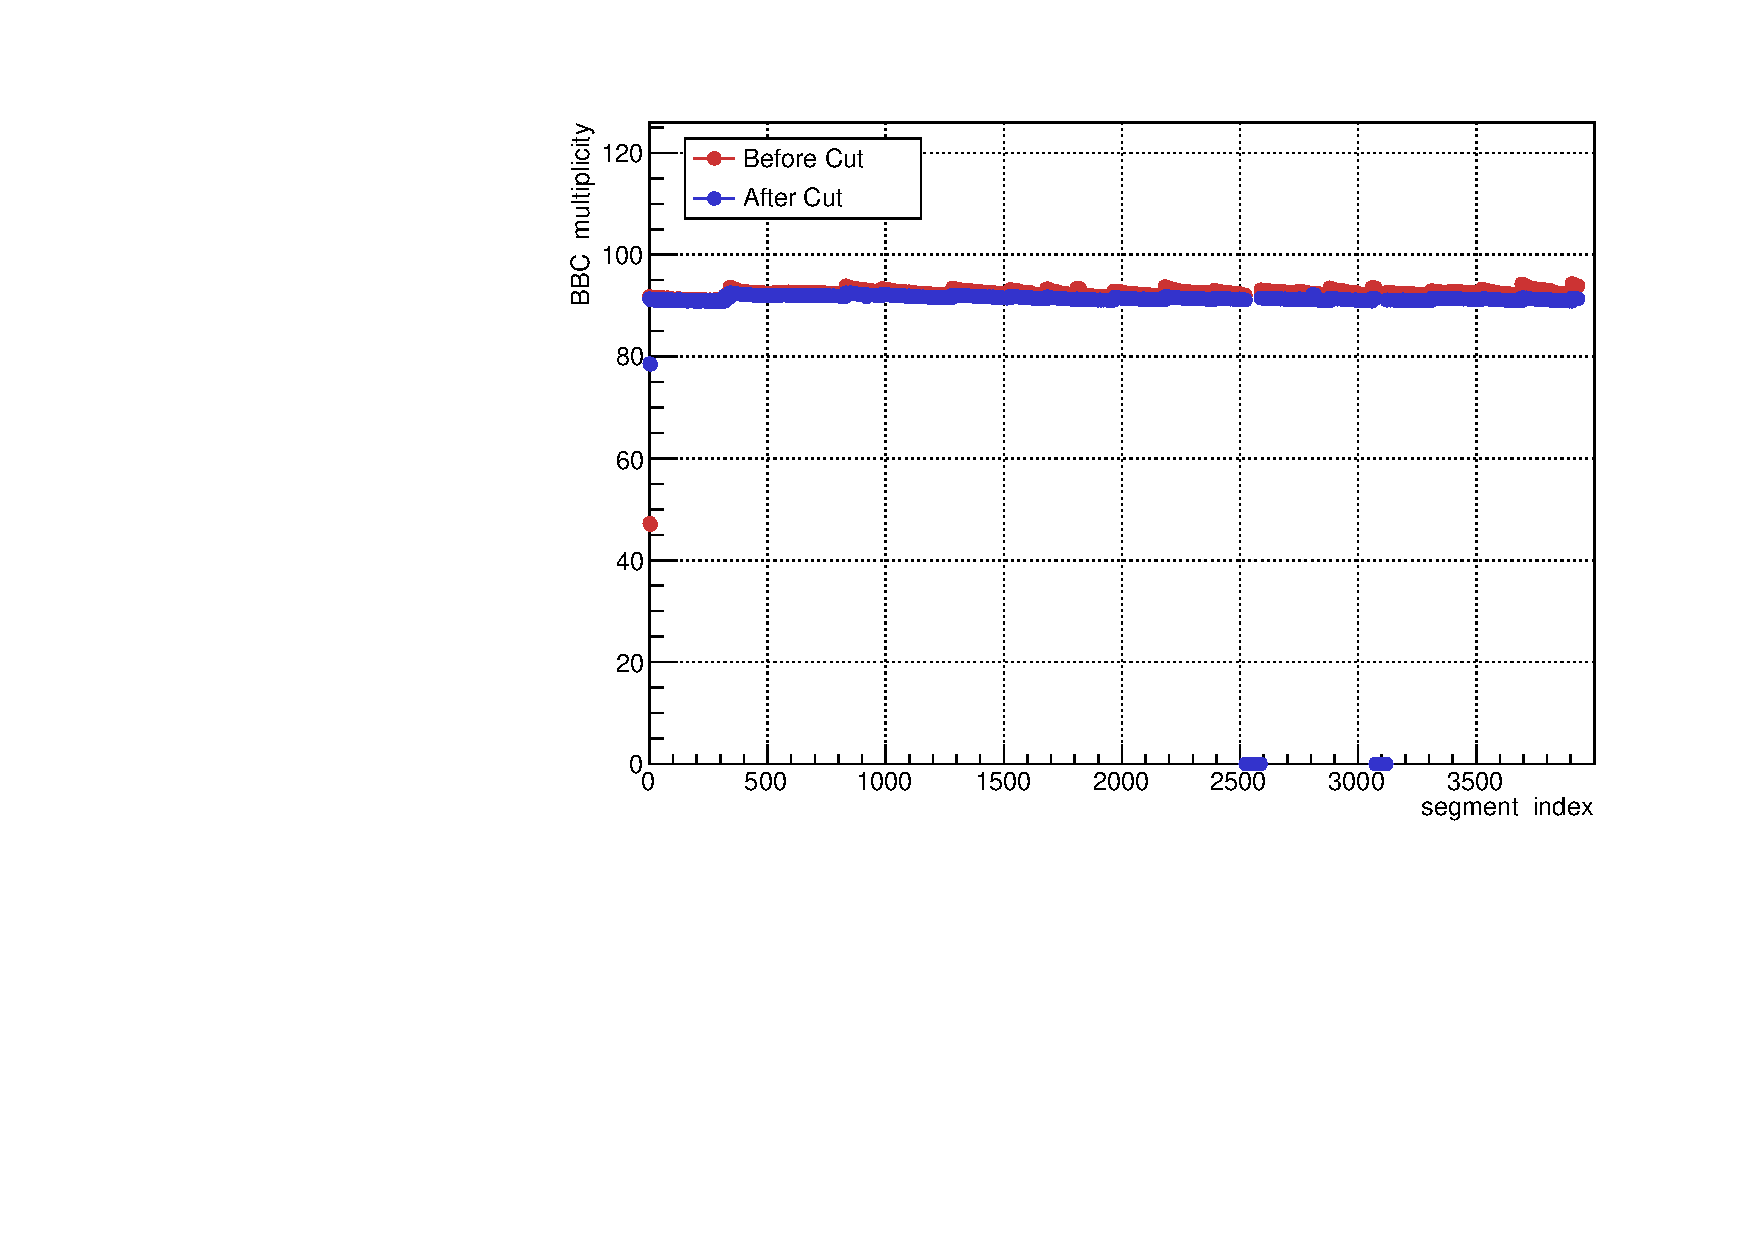
\includegraphics[width=\textwidth]{fig_pileup/dAu200MB_TimingBBC_BBCM}\\
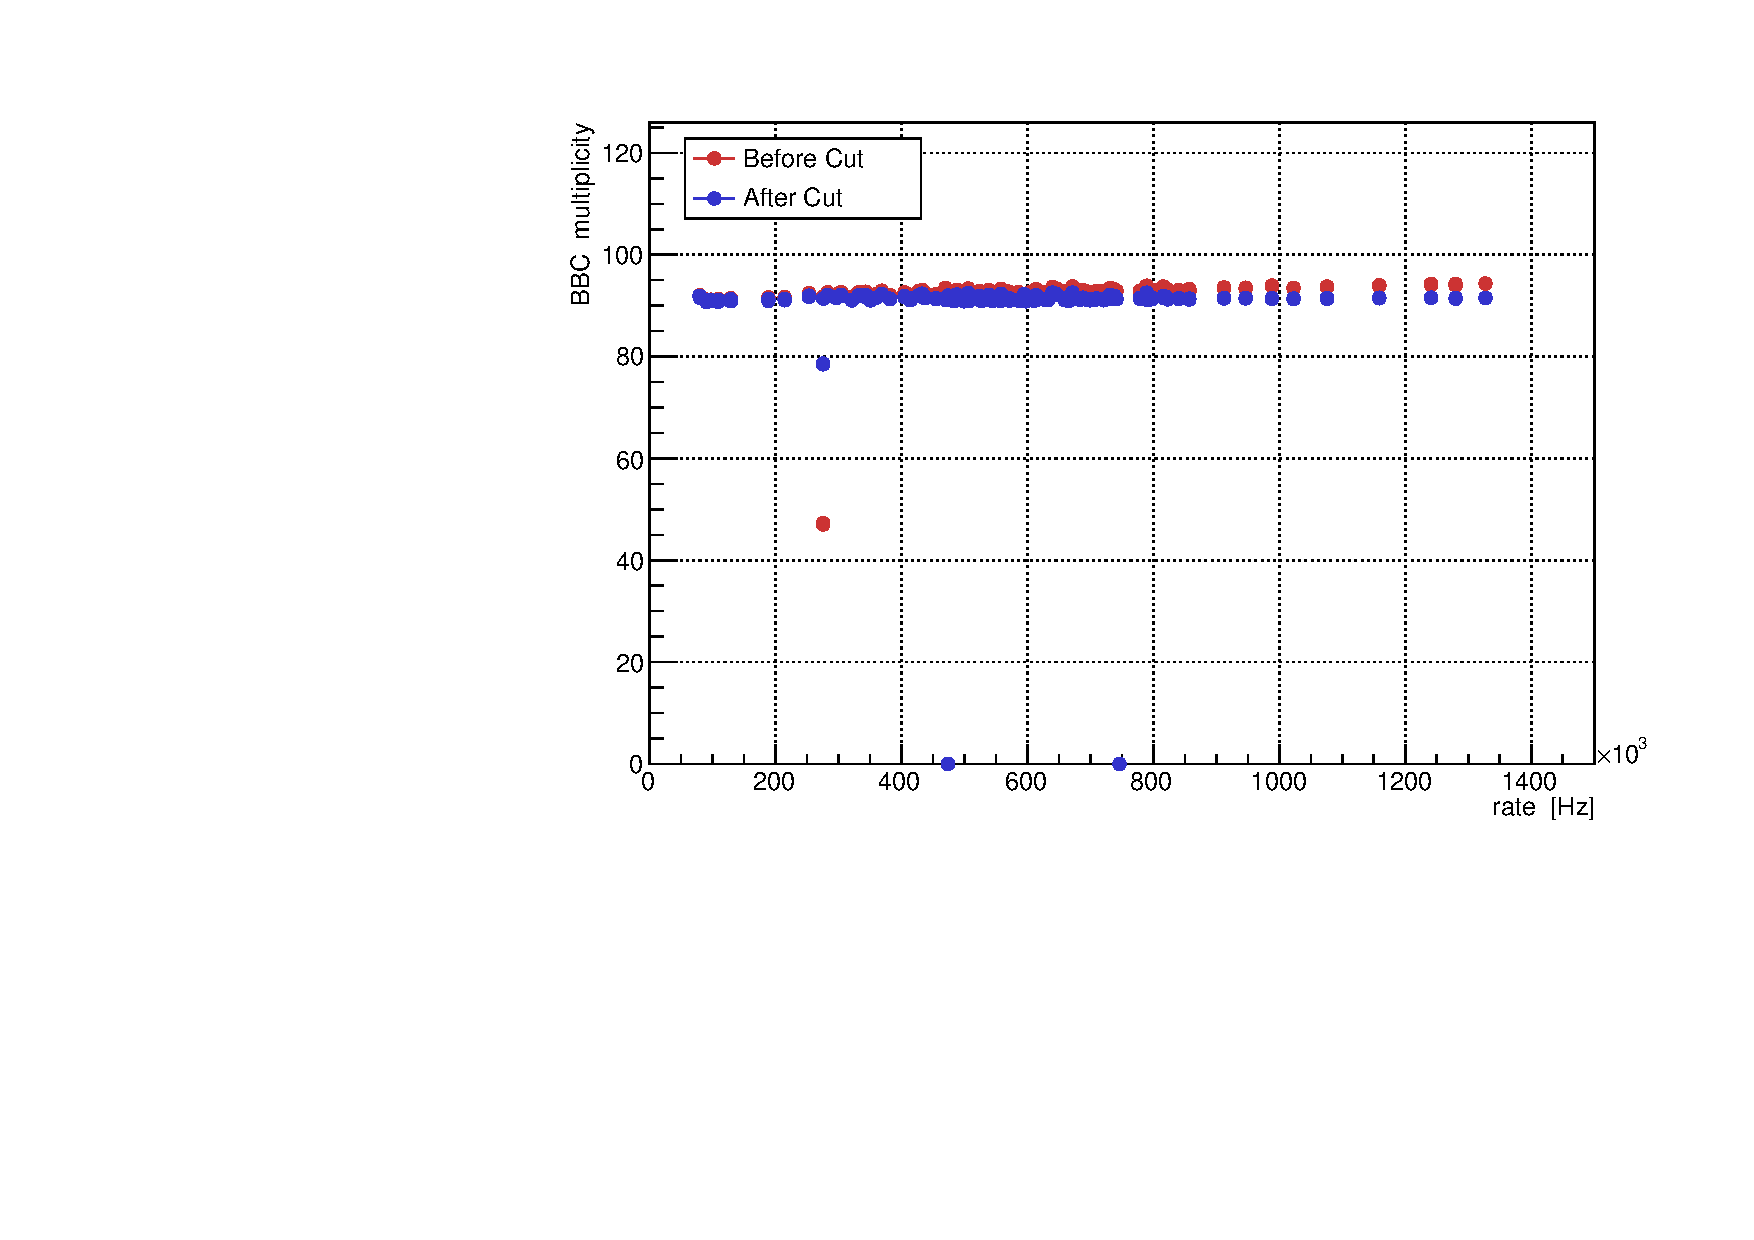
\includegraphics[width=\textwidth]{fig_pileup/dAu200MB_TimingBBC_RATEBBCM}
\label{fig.dau200mb.bbcrate}
\caption{Performance of the pileup rejection cut in dAu 0-5\% centrality class. The top plot correspond tot he the total BBCsouth signal as a function of time (the analysis was done for each run segment). The bottom plot is the depedence of the BBCsouth signal run by run to the total instantanoeus rate.}
\end{figure}


%\bibliography{references}{}
%\bibliographystyle{plain}
\end{document}

